
\lhead[\chaptername~\thechapter]{\rightmark}

\rhead[\leftmark]{}

\lfoot[\thepage]{}

\cfoot{}

\rfoot[]{\thepage}

\chapter{Related Work}
\label{related}

Since our idea of using diverse user requirements to personalize the systems for efficiency is applied to both image classification and image retrieval tasks, related work of both tasks will be provided in their respective sections.

\section{Image Classification}

Our proposed method is to obtain a CNN model that can be used partially by each user according to their requirements to be able to distribute efficient models to each user.
As our proposed method aims for efficiency, efficient CNNs will be the main topic in this section.
In the following subsections, efficient CNN models such as various compression methods will be mentioned.
More emphasis will be done to dynamic compression methods.
Moreover, our proposed method is using a hierarchical approach to solve the problem. 
Because of this, we will also address some hierarchical systems that are similar to our proposed model.

\subsection{Efficient CNNs}

Deep neural network compression techniques reduce the size of the neural networks for a considerable amount. 
There has been much research about how to efficiently compress neural networks, examples of such methods include pruning~\cite{anwar2017structured}, quantization~\cite{han2016eie}, knowledge distillation~\cite{hinton2015distilling} etc. 
Generally, compression methods prioritize either memory, computation or energy cost while obtaining more efficient CNN models.

\begin{figure}
    \centering
    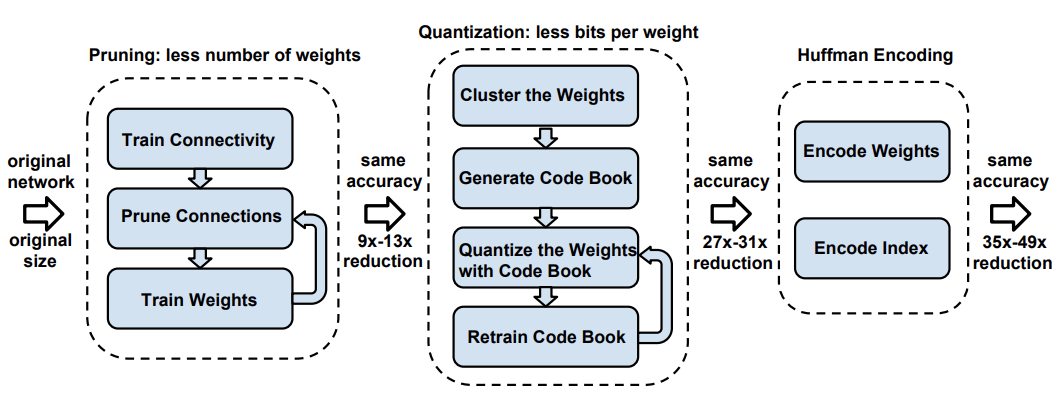
\includegraphics[width=\textwidth]{thesis/images/deep_comp-fig.png}
    \caption{Three steps of Deep Compression by Han et al.~\cite{han2015deep}}
    \label{fig:deepcomp}
\end{figure}

Pruning CNN models involves eliminating some individual connections~\cite{molchanov2016pruning} \cite{Yu_2018_CVPR} \cite{Wang2018StructuredPP} or discarding entire channels~\cite{He_2017_ICCV}~\cite{li2016pruning} that are identified as having a small importance on the output result.
In a famous work about pruning~\cite{han2015deep}, Han \emph{et al.} succeeded to reduce the size of VGG-16 by 49x with a 3-step method, as in figure \ref{fig:deepcomp}. 
First step is to prune or eliminate the model connections whose weights are below a threshold. 
In this step, the remaining connections are needed to be re-trained for a couple of epochs to maintain the accuracy.
The next step is quantization by grouping the remaining weights into shared weights to reduce the bits to represent the all of the weights.
Last step is using Huffman coding to further reduce the bit representation of all the weights. 
Another way of reducing the model size is knowledge distillation. 
One highly influential example is the work by Hinton \emph{et al.}, where the main idea is to use the output of a large model or an ensemble of specialist models to train a compact network while retaining the accuracy.
Instead of training from the data with definite one-hot coded labels, a larger model is imitated by training a smaller one with the probabilistic outputs of the large model.
In this way, a larger model is condensed into a smaller version.

Not only all the above-mentioned methods require a costly re-training phase to maintain the accuracy,
but also they reduce the size of the model in general, not with respect to each user's requirements of using the model. 
Moreover, our method is to allow users to adaptively use part of the functionality of a model instead of a compression technique.
Having said that, our method can be used jointly with the mentioned works for further reducing the size of the models according to user requirements.

\subsection{Dynamic Approaches}

More dynamic approaches include pruning convolutional channels at runtime depending on the input image supported by a RNN network to decide which channels to be omitted~\cite{Lin2017RuntimeNP}. 
As in the figure \ref{fig:runtimenp}, some feature maps are being omitted according to the input image and previously omitted feature maps supervised by RNN.
This method preserves the full ability of the network and improves the speed of the network while maintaining the accuracy. 
The network runs adaptively according to each input images by only activating relevant feature maps while forwarding an image.
However, the model is not getting smaller in storage size as the whole model remains in the device. 
As one of our concern is the restricted storage memory of wearable devices, it does not serve our purpose of providing users with smaller models custom-made for their requirements. 

\begin{figure}
    \centering
    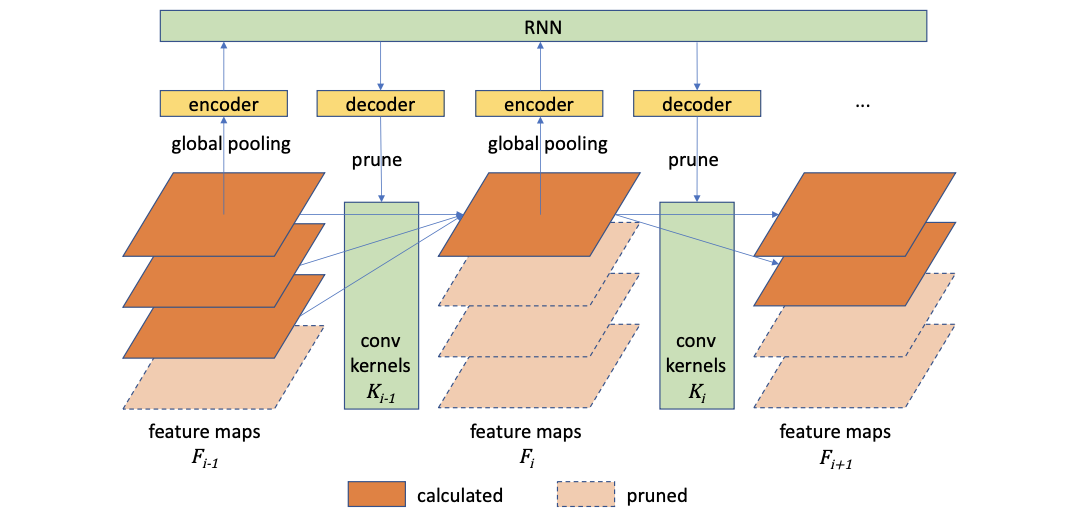
\includegraphics[width=\textwidth]{thesis/images/runtimenp-fig.png}
    \caption{Overall framework of Runtime Neural Pruning~\cite{Lin2017RuntimeNP}}
    \label{fig:runtimenp}
\end{figure}

Another method, namely AdaDeep~\cite{Liu2018OnDemandDM}, automatically selects a combination of compression techniques especially for deploying neural networks on resource-constrained mobile platforms. 
AdaDeep aims to compress CNN models according to user specifications such as memory limitation, desired accuracy, etc. 
It chooses the best combination of compression algorithms among many different algorithms that prioritize different aspects according to user-specified performance goals and resource constraints. 
Despite serving each user personalized compression, this method is not for adaptively using a sub-functionality of the model.
The resulting model has all the classification functionality that the user does not need for their usage purposes. 
Even though this method satisfies each user's system requirements, it is not removing the undesired functionality of the system to reduce the network size.

A method for on-device customization of CNNs~\cite{guo2017pruning2} aims to prune the unneeded classes with their corresponding filters according to user needs. 
For each class labels, they calculate the impact of each filters on the class labels. 
Not only do they compute impact of each filter on each class, they also compute the compensation needed by the linear combination of other filters.
In their scenario, the system distributes the model to each user with an automatic pruning algorithm tailored to each user's need. 
Then, the users can prune the filters in the model for a specific subset of classes and apply the compensation algorithm to maintain the accuracy after pruning. 
As all of the calculation is done beforehand, the user just needs to run the program without the need for re-training or fine-tuning.
A later work of the same group~\cite{guo2017pruning} changes the compensation method.
The new compensation parameters are either the mean feature map or the feature map of the most correlated filter.
The experiments are only done in CIFAR-10 dataset. The classification accuracy is compared between 10-class model a few-class models, so it is hard to analyze the accuracy drop.
Moreover, according to their scenario, the whole model is loaded to user's device which might be a memory issue.
Also, there is still compensation algorithm required to be run on user-side, whereas in our method users do not need to change the model once the model is loaded.

\subsection{Hierarchical Solutions}

There is plenty of work adopting hierarchically structured CNNs. 
While some of them employ the hierarchy to achieve higher accuracy, the others aim to obtain efficient models.
Roy \emph{et al.}~\cite{roy2018tree} uses a Tree-CNN to propose a solution for incremental learning. 
In their architecture, the branches of the network grows as new classes added to the model without having an effect on the already learned classes. 
This hierarchical model is quite similar to our proposed model in this paper, regardless of the problem that it solves. 
HD-CNN~\cite{Yan_2015_ICCV} approaches image classification with the idea that some classes are easy to classify and they only need coarse networks while others require deeper and more complicated networks. 
They make use of a hierarchical classifier to classify easy and hard images on different levels to improve better accuracy. 

Below methods use hierarchical decomposition to convert large networks into small few-class networks.
In \cite{chennupati2016hierarchical} and \cite{nooka2016adaptive}, the aim is to divide the functionality of a large deep network into multiple smaller networks. 
They use an interesting way of clustering the labels according to the similarities between them, using confusion matrix for the classification of these labels.
Then, multiple smaller parallel-working networks are obtained. 
Their results are combined to have the overall result for the classification of all labels.
With this method, individual models can be used for classifying a subset of classes.
However, the class labels in sub-models are fixed as the decomposition of the large model is based on the similarity of the labels instead of the actual user requirements.
HSD-CNN~\cite{sairam2018hsd} successfully converts many-class CNN to a hierarchical model by branching the network to two after some initial layers.
While branching, the class set is divided to two subsets according to their similarity.
The layers are split according to their impact on the score for both subsets.
The resulting network needs fine-tuning step for a few epochs at the end. 
Moreover, the class separation is done according to the similarities of the labels instead of considering the user requirements.
Even though, there are various usage of hierarchical CNNs, we believe it is a novel approach to exploit them for allowing users to adaptively use sub-parts of the model according to their individual requirements.


\section{Image Retrieval}

The aim of image retrieval task is to find the closest vector to a query image in a search database, where images are represented by descriptor vectors.
Because the cost of finding the nearest vector is high with traditional algorithms, Approximate Nearest Neighbor (ANN) search is being used for many practical applications.
Our proposed method is built on ANN algorithm to further reduce the area of search space according to user requirements. 
In the following subsections, firstly, various ways of obtaining descriptor vectors from the images will be mentioned. 
Then, recent fast and efficient ANN algorithms will be discussed thoroughly. 

\subsection{Obtaining Descriptors}

Before the arrival of neural networks, SIFT features were mainly used to obtain descriptor vector for the images~\cite{philbin2007object}~\cite{jegou2010aggregating}. 
However, CNN-based descriptors quickly substituted the traditional methods. 
Zheng \emph{et al.} compared the performance of many SIFT-based and CNN-based methods on various datasets and superiority of CNN-based methods can clearly be seen. 
Conventional CNN-based methods use a pre-trained model and they take the output of one of the last fully connected layers as the descriptor vector. 
In \cite{babenko2014neural}, they compare the descriptor vectors obtained by the output of different last layers of CNN to see which layer is the best for descriptors.
It is also shown that training the CNN for classification task on a different dataset such as ImageNet gives fairly good results, while fine-tuning the model on the retrieval dataset gives better results.
Later works use only convolutional layers with a following global pooling operation~\cite{razavian2016visual}~\cite{tolias2015particular}. 
In a recent state-of-the-art paper for deep global image descriptor~\cite{radenovic2018fine}, descriptor vectors are obtained with convolutional layers followed by a generalized mean pooling operation.

When obtaining descriptor vectors, one should consider the curse of dimensionality. 
As the dimensions of the output layer of CNN can be quite large, most recent works apply whitening with principal component analysis. 
In \cite{jegou2012negative}, whitening is proved to be beneficial and actually improve the accuracy of the retrieval task.

In our work, we simply used VGG-16~\cite{simonyan2014very} pre-trained on ImageNet with the last fully connected layer removed to obtain descriptor vectors. PCA whitening is also applied to reduce the dimension to 64.

\subsection{Approximate Nearest Neighbor Search}

\subsubsection*{Hashing-based methods}

Generally in hashing methods, all database vectors and the query vectors are mapped to lower dimension vectors called \emph{hash-codes} by using several hash functions and the actual search depends on the method. 
In the methods using hash tables and inverted lists, such as Locality Sensitive Hashing (LSH)~\cite{indyk1998approximate}, every hash table has inverted lists on their indices containing the database vectors that falls into one of the lists when the hash function is applied.
Then, only the vectors that are mapped to the same code as the query vector are searched, therefore only a few inverted lists are checked.
On the other hand, other methods compare hash-codes of query and database vectors directly to find the nearest vector.
However, these methods were highly sensitive to data distribution as hash functions should be carefully chosen according to the data. 
As a result, learning-based hashing methods are appeared~\cite{weiss2009spectral}~\cite{liu2012supervised}.
There are many different hashing methods based on LSH, varying by the distance or similarity calculation.

\subsubsection*{Quantization-based methods}
\label{subsec:related-quantization}

\begin{figure}
    \centering
    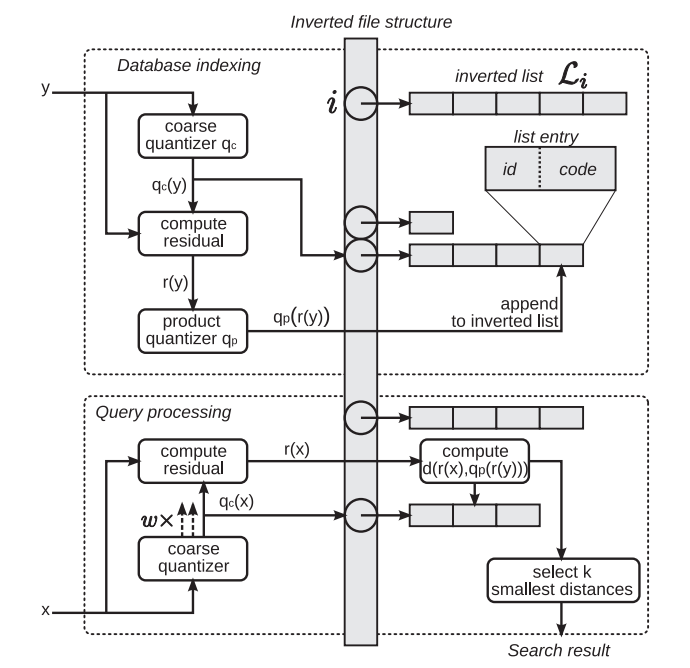
\includegraphics[width=.6\textwidth]{thesis/images/pq-fig.png}
    \caption{Inverted list scheme of Product Quantization\cite{jegou2010product}}
    \label{fig:pq}
\end{figure}

LSH-based methods were outperformed by quantization-based methods, especially for larger-scale data due to their huge memory cost.
In Product Quantization (PQ)~\cite{jegou2010product}, vectors are again mapped to lower dimension vectors to reduce memory consumption. 
However, the number of possible distances, hence the accuracy, is much higher than LSH-based methods using Hamming distance~\cite{weiss2009spectral}.
Moreover, the distances between vectors and the short codes can be calculated fast and accurately.
An inverted list structure, as in figure \ref{fig:pq}, is used to limit the comparison with only the most relevant vectors.

In PQ, search space (database) is divided by using k-means clustering and each quantized database vector are assigned to their respective clusters using euclidian distance. 
Note that, short-coded database vectors are stored with their distance to their respective cluster centroids in their inverted lists, so that the distance can be used to efficiently calculate the closest short code to the query vector.
Quantization of the vectors works as follows.
The vector with dimension $D$ is split into $m$ sub-vectors with same smaller dimensions, $D/m$, and each sub-vector is quantized with different quantizers according to the codebook. 
This quantization scheme reduce the size of the vectors for a great amount.
The search is performed between the query vector and quantized vectors, called Asymmetric Distance Calculation (ADC) instead of quantized query vector and quantized database vectors because Jegou \emph{et al.} showed estimated distances with ADC overlaps more with the true distances.
After finding the closest centroid to the query vector, its distance to the centroid is compared with the distances of the database vectors belonging to that centroid. 
The smallest difference between the distances gives the closest vector.

There are several works that improved product quantization. Optimized Product Quantization (OPQ)~\cite{ge2013optimized} changes the problem into an minimization problem of quantization error(lost information with quantization) and optimize codebooks to improve accuracy of PQ with more computational cost. 
On the other hand, Composite Quantization (CQ)~\cite{wang2018composite} uses composition of $m$ elements to represent a vector instead of splitting the vector to $m$ equal parts. 
Sub-codewords are added instead to reconstruct the vector. 
Reconstruction error and accuracy is better than that of PQ with additional computational cost.

In our work, we used PQ with inverted list as a baseline for approximate nearest neighbor search. 
We specifically improved the first part of the search where the query vector is compared with the centroids by reducing the number of centroids to check with respect to the user requirements. 

\begin{figure}
    \centering
    \begin{subfigure}[b]{0.4\textwidth}
        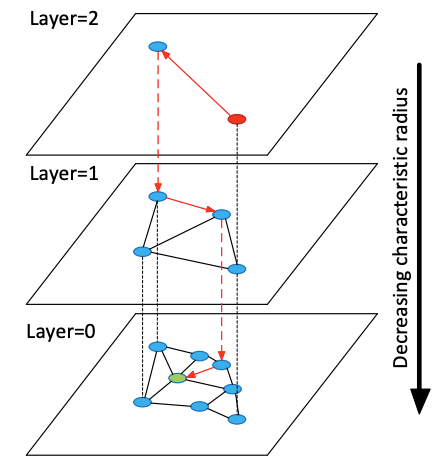
\includegraphics[width=\textwidth]{thesis/images/hnsw-fig.png}
        \caption{The search starts from the top layer with longer connections and continues to lower layers when a local minimum is found.}
        \label{fig:hnsw1}
    \end{subfigure}
  %
    \begin{subfigure}[b]{0.45\textwidth}
        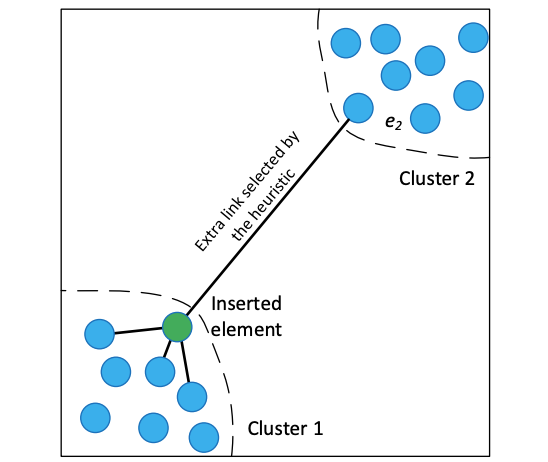
\includegraphics[width=\textwidth]{thesis/images/hnsw-fig2.png}
        \caption{Heuristic chooses an element from another cluster, if inserted element is the closest to $e_2$ compared to other nodes in Cluster 1.}
        \label{fig:hnsw2}
    \end{subfigure}
    \caption{Hierarchical Navigable Small World~\cite{malkov2018efficient}}
    \label{fig:hnsw}
\end{figure}

\subsubsection*{Graph-based methods}

In graph-based methods, search space is represented with a graph, where the nodes are the database vectors. 
Graph is traversed in a greedy manner to find the closest node to the query vector.
As the database vectors are added to the graph, each node is connected to a few neighboring nodes.
At the beginning of constructing the graph, edges between the few starting nodes are expected to be longer because the probability of finding smaller nodes to connect is higher near the end of construction.
These longer edges are important for fast efficient search.
State-of-the-art work on approximate nearest neighbor search uses an improved version of a graph, namely hierarchical navigable small world (HNSW)\cite{malkov2018efficient}. 
Other NSW methods all suffer from search complexity and scalability. 
HNSW solves the issue by separating the graph into different layers according to the length of the links between the nodes as in figure \ref{fig:hnsw1}. 
Thus, only a fixed number of connections needs to be evaluated for each step because of the hierarchy, which results in a better scalability.
They proposed starting the search from the layer with the longest links to not be stuck in a false local minima. 
The greedy search starts from the upper layers with longer links and continues iteratively towards the lower layers with shorter links when a local minimum is reached.
One other strategy to maintain global connectivity is to add connections between separated clusters with an advanced heuristic\ref{fig:hnsw2}. 
While adding a node to the graph, instead of just connecting the nearest neighbors, an extra link is created to a node in another cluster to improve graph connectivity, therefore improving the probability of traversing until the closest node.

